% Ensure xcolor receives the `table` option before any package/class loads it
\PassOptionsToPackage{table}{xcolor}
\documentclass[aspectratio=169,10pt]{beamer}

% ===============================
% Hochschule Aalen Look & Feel
% ===============================
\usepackage[T1]{fontenc}
\usepackage[utf8]{inputenc}
\usepackage[ngerman]{babel}
\usepackage{lmodern}
\usepackage{graphicx}
\usepackage{booktabs}
\usepackage{hyperref}
% xcolor options are passed above to avoid option clash with class/packages
\usepackage{xcolor}
\usepackage{csquotes}
\usepackage{listingsutf8}
\usepackage{colortbl}
\usepackage{array}
\usepackage{tabularx}

\definecolor{hsaaBlue}{RGB}{0,70,135}
\definecolor{hsaaGray}{RGB}{100,100,100}

\usetheme{default}
\usecolortheme{default}
\setbeamertemplate{navigation symbols}{}

\setbeamercolor{normal text}{fg=black,bg=white}
\setbeamercolor{structure}{fg=hsaaBlue}
\setbeamercolor{frametitle}{fg=hsaaBlue,bg=white}
\setbeamerfont{frametitle}{series=\bfseries,size=\large}

\lstset{
  inputencoding=utf8,
  basicstyle=\ttfamily\footnotesize,
  keywordstyle=\color{hsaaBlue},
  commentstyle=\color{hsaaGray},
  showstringspaces=false,
  frame=single,
  breaklines=true,
  literate={ä}{{\"a}}1{ö}{{\"o}}1{ü}{{\"u}}1{Ä}{{\"A}}1{Ö}{{\"O}}1{Ü}{{\"U}}1{ß}{{\ss}}1
}

\newcolumntype{Y}{>{\raggedright\arraybackslash}X}

\newcommand{\hsaaLogo}{%
  \IfFileExists{Hochschule-aalen.svg.png}{%
    
\includegraphics[height=0.9cm]{Hochschule-aalen.svg.png}%
  }{%
    \IfFileExists{hs-aalen-logo.png}{\includegraphics[height=0.9cm]{hs-aalen-logo.png}}{}%
  }%
}

\setbeamertemplate{headline}{%
  \begin{beamercolorbox}[wd=\paperwidth,ht=1.15cm,dp=0pt]{normal text}%
    \vbox to 1.15cm{%
      \vfil
      \hbox to \paperwidth{\hspace*{0.6cm}\hfill\hsaaLogo\hspace*{0.6cm}}%
      \vfil
    }%
  \end{beamercolorbox}%
  \nointerlineskip%
  {\color{hsaaBlue}\rule{\paperwidth}{1.2pt}}%
}

\setbeamercolor{footline}{bg=hsaaBlue,fg=white}
\setbeamerfont{footline}{size=\scriptsize}
\setbeamertemplate{footline}{%
  \begin{beamercolorbox}[wd=\paperwidth,ht=3.4ex,dp=1.1ex,leftskip=0.8cm,rightskip=0.8cm]{footline}%
    \insertdate{} \textbullet\ \insertshortauthor{} \textbullet\ Master Informatiker\hfill\insertframenumber{} / \inserttotalframenumber
  \end{beamercolorbox}%
}

% ===============================
% Titelinformationen
% ===============================
\title[Strategized Locking Pattern]{Strategized Locking Pattern}
\subtitle{Pattern-Oriented Software Architecture, Vol.~2 (POSA2)}
\author[Florian Merlau]{Florian Merlau}
\institute[]{Master Informatik -- Advanced Software Quality (WiSe 25/26)}
\date{\today}
\setbeamerfont{title}{series=\bfseries,size=\Huge}
\setbeamerfont{subtitle}{series=\mdseries,size=\large}
\setbeamerfont{author}{size=\normalsize}
\setbeamerfont{institute}{size=\normalsize}
\setbeamerfont{date}{size=\normalsize}

\makeatletter
\setbeamertemplate{title page}{%
  \vspace*{5cm}%
  \begin{beamercolorbox}[wd=\paperwidth,ht=0pt,dp=0pt,leftskip=2.4cm,rightskip=2.4cm]{normal text}%
    \centering
    {\usebeamerfont{title}\color{hsaaBlue}\inserttitle\par}%
    \vspace*{0.6cm}%
    {\usebeamerfont{subtitle}\color{hsaaGray}\insertsubtitle\par}%
    \vspace*{1.2cm}%
    {\usebeamerfont{author}\insertauthor\par}%
    {\usebeamerfont{institute}\insertinstitute\par}%
    \vspace*{0.8cm}%
    {\usebeamerfont{date}\insertdate\par}%
  \end{beamercolorbox}%
  \vfill
}
\makeatother

\begin{document}

\begin{frame}
  \titlepage
\end{frame}

\begin{frame}{Agenda}
  \tableofcontents[hideallsubsections]
\end{frame}

% ===============================
% Einleitung & Motivation
% ===============================
\section{Einf\"uhrung \& Motivation}
\begin{frame}{Motivation}
  \begin{itemize}
    \item Nebenl\"aufige Software ist fehleranf\"allig: \textit{Race Conditions, Deadlocks}
    \item Feste Locking-Strategien sind unflexibel und schwer wartbar
    \item Ziel: Wiederverwendbare Komponenten mit austauschbaren Synchronisationsmechanismen
  \end{itemize}
\end{frame}

\begin{frame}{Problem klassischer Ans\"atze}
  \begin{itemize}
    \item Hard-coded Locks $\rightarrow$ geringe Flexibilit\"at
    \item Mehrere Varianten desselben Codes f\"ur unterschiedliche Threading-Modelle
    \item Schwierige Wartung, fehleranf\"allig, Performance-Verlust
  \end{itemize}
\end{frame}

% ===============================
% Patternbeschreibung
% ===============================
\section{Patternbeschreibung}
\begin{frame}{Intent und Kontext}
  \textbf{Intent:}\\
  \textit{Strategize a component's synchronization to increase its flexibility and reusability without degrading performance or maintainability.} (Schmidt, 1998)

  \vspace{1em}
  \textbf{Kontext:}
  \begin{itemize}
    \item Wiederverwendbare Komponenten, die in verschiedenen Concurrency-Umgebungen laufen m\"ussen
    \item Locking soll konfigurierbar oder \enquote{pluggable} sein
  \end{itemize}
\end{frame}

\begin{frame}{Problem \& Forces}
  \begin{itemize}
    \item Unterst\"utzung verschiedener Locking-Strategien (Mutex, RW-Lock, Null-Mutex)
    \item Anforderungen: Performance, Wartbarkeit, Portabilit\"at
    \item Trade-off: Compile-Time Templates vs. Run-Time Polymorphie
  \end{itemize}
\end{frame}

\begin{frame}{L\"osung -- Strategized Locking}
  \begin{itemize}
    \item Synchronisation wird ausgelagert in eine Strategie-Komponente
    \item Zwei Varianten:
      \begin{enumerate}
        \item \textbf{Polymorph} -- Lock-Typ wird zur Laufzeit gew\"ahlt
        \item \textbf{Template-basiert} -- Lock-Typ wird beim Kompilieren festgelegt
      \end{enumerate}
    \item Nutzung des \textbf{Scoped Locking Idioms} (RAII)
  \end{itemize}
\end{frame}

% ===============================
% Codebeispiel & Diagramm
% ===============================
\section{Codebeispiel und Diagramm}
\begin{frame}[fragile]{Codebeispiel (C++)}
\begin{lstlisting}[language=C++]
template <class LOCK>
class File_Cache {
public:
  const char* find(const char* path) {
    Guard<LOCK> guard(lock_);
    // Zugriff auf Cache...
    return nullptr;
  }
private:
  LOCK lock_;
};
\end{lstlisting}
\end{frame}

\begin{frame}{Diagramm -- Strategized Locking}
  \begin{center}
     \begin{figure}
      \centering
      % Include the UML diagram if present (use a moderate width). If the file is
      % missing, show a framed placeholder.
      \IfFileExists{UML-Klasse.pdf}{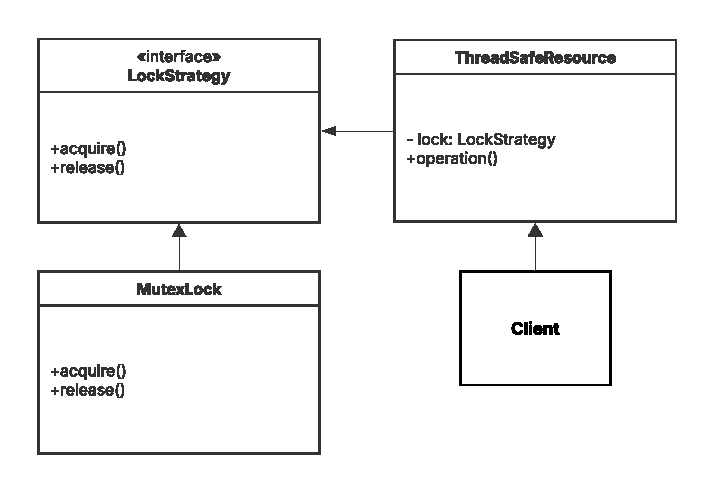
\includegraphics[width=0.55\linewidth,keepaspectratio]{UML-Klasse.pdf}}{\fbox{Diagramm fehlt (UML-Klasse.pdf)}}

      % Caption / Bildunterschrift: kleine, kursive Beschreibung
      \vspace{0.6em}
      {\footnotesize\itshape Abbildung: Eigene Darstellung des Klassendiagramms zur Strategized Locking.}

      % Autor-/Signaturlinie rechtsbündig in dezenter Farbe
      \vspace{0.4em}
      {\raggedleft\scriptsize\textcolor{hsaaGray}}
     \end{figure}
  \end{center}
\end{frame}

\begin{frame}{Vergleich der Strategien}
  \centering
  {\small
  \setlength{\tabcolsep}{6pt}
  \renewcommand{\arraystretch}{1.25}
  \arrayrulecolor{hsaaGray!40}
  \begin{tabularx}{0.92\linewidth}{>{\bfseries}lYYY}
    \toprule
    \rowcolor{hsaaGray!25}
    Strategie & Beschreibung & Vorteil & Nachteil \\
    \midrule
    \rowcolor{hsaaGray!10}
    Null\_Mutex & Kein Lock (Single-Threaded) & Schnell & Unsicher bei Threads \\
    Thread\_Mutex & Standard-Lock & Robust & Langsam bei hoher Parallelit\"at \\
    \rowcolor{hsaaGray!10}
    RW\_Lock & Paralleles Lesen, exklusives Schreiben & Effizient bei vielen Reads & Komplexer \\
    \bottomrule
  \end{tabularx}
  \arrayrulecolor{black}}
\end{frame}

% ===============================
% Verwandte Patterns
% ===============================
\section{Verwandte Patterns}
\begin{frame}{Thread-safe Interface Pattern}
  \begin{itemize}
    \item Verhindert \textit{Self-Deadlocks} durch klare Trennung
    \item \textbf{Interface methods check} -- \"offentliche Methoden sichern Zugriff
    \item \textbf{Implementation methods trust} -- interne Methoden vertrauen auf bestehenden Lock
  \end{itemize}
\end{frame}

\begin{frame}[fragile]{Scoped Locking Idiom}
  \begin{itemize}
    \item RAII-Prinzip: Lock wird beim Eintritt erworben, beim Verlassen freigegeben
  \end{itemize}
  \vspace{1em}
  \begin{lstlisting}[language=C++]
template<class LOCK>
class Guard {
public:
  Guard(LOCK &l): lock(l) { lock.acquire(); }
  ~Guard() { lock.release(); }
private:
  LOCK &lock;
};
  \end{lstlisting}
\end{frame}

% ===============================
% Bewertung & Fazit
% ===============================
\section{Bewertung \& Fazit}
\begin{frame}{Vor- und Nachteile}
  \textbf{Vorteile:}
  \begin{itemize}
    \item Hohe Flexibilit\"at und Wiederverwendbarkeit
    \item Wartungsfreundlich (eine zentrale Implementierung)
    \item Einfache Performance-Anpassung
  \end{itemize}
  \vspace{1em}
  \textbf{Nachteile:}
  \begin{itemize}
    \item Template-Komplexit\"at bzw. Sichtbarkeit der Strategien
    \item Potenziell h\"ohere Kompilierzeit
  \end{itemize}
\end{frame}

\begin{frame}{Bekannte Anwendungen}
  \begin{itemize}
    \item \textbf{ACE Framework (Adaptive Communication Environment)}
    \item \textbf{Booch Components}
    \item Moderne \"Aquivalente: \texttt{std::lock\_guard}, Java \texttt{synchronized}
  \end{itemize}
\end{frame}

\begin{frame}{Fazit}
  \begin{itemize}
    \item Strategized Locking = ``pluggable synchronization''
    \item Klare Trennung von Funktionalit\"at und Synchronisation
    \item Grundlage vieler moderner Concurrency-Patterns
  \end{itemize}
\end{frame}

\begin{frame}{Diskussion}
  \begin{itemize}
    \item Wann lohnt sich Strategized Locking in modernen Systemen?
    \item Welche Alternativen gibt es in Java, C++, Rust?
  \end{itemize}
\end{frame}

% ===============================
% Quellen
% ===============================
\begin{frame}[allowframebreaks]{Quellen}
  \begin{thebibliography}{9}
  \bibitem{schmidt1998}
    Douglas C. Schmidt,
    \emph{Strategized Locking, Thread-safe Interface, and Scoped Locking},
    C++ Report, Washington University, 1998.
  \bibitem{buschmann2000}
    Buschmann, F., Schmidt, D. C., et al.
    \emph{Pattern-Oriented Software Architecture, Volume 2: Patterns for Concurrent and Networked Objects.}
    Wiley, 2000.
  \end{thebibliography}
\end{frame}

\end{document}
